%REPORT TEMPLATE
%AUTHOR: RUI QU  
%EMAIL: RQU@KTH.SE 

%----------------------------------------------------------------------------------------
%	PACKAGES AND DOCUMENT CONFIGURATIONS
%----------------------------------------------------------------------------------------

\documentclass{article}

%---Basic---
\usepackage{natbib} % Required to change bibliography style to APA
\usepackage{amsmath} % Required for some math elements 
\setlength\parindent{0pt} % Removes all indentation from paragraphs
\usepackage{listings}%Insert code
\usepackage{times} % Uncomment to use the Times New Roman font

%---Table---
\usepackage{multirow}%Table
\usepackage{booktabs}%Table Triple-lines
\usepackage{siunitx} % Provides the \SI{}{} and \si{} command for typesetting SI units

%---Figure---
\usepackage{graphicx} % Required for the inclusion of images
\usepackage{subfigure} % Required for multiple images
\usepackage{float} 

%---Pseudo-code in LaTeX---
\usepackage{minted} %Preference->engine->pdfTeX->Latex  ADD: -shell-escape
\usepackage{xcolor}
\definecolor{bg}{rgb}{0.95,0.95,0.95}

\usepackage{algorithm}
\usepackage{algpseudocode}
\usepackage{amsmath}
\renewcommand{\algorithmicrequire}{\textbf{Input:}}  % Use Input in the format of Algorithm
\renewcommand{\algorithmicensure}{\textbf{Output:}} % Use Output in the format of Algorithm

%---Appendix---
\usepackage{appendix}
\newcommand{\upcite}[1]{\textsuperscript{\textsuperscript{\cite{#1}}}} %Upcite

%----------------------------------------------------------------------------------------
%	DOCUMENT INFORMATION
%----------------------------------------------------------------------------------------

\begin{document}

\title{CS-E5710 Bayesian Data Analysis\\Assignment 7}                  
%\author{Rui Qu\\rui.qu@aalto.fi}
\maketitle

% If you wish to include an abstract, uncomment the lines below
% \begin{abstract}
% Abstract text
% \end{abstract}

%----------------------------------------------------------------------------------------
%	SECTION 1
%----------------------------------------------------------------------------------------

\textbf{Note: }Complete source code is given in the Appendix.

\section{Linear model: drowning data with Stan}

\begin{minted}[bgcolor=bg, linenos, fontsize=\footnotesize]{python}  
drowning_data = pd.read_fwf('./drowning.txt').values
years = drowning_data[:, 0]
drowning = drowning_data[:, 1]
plt.plot(years, drowning)
print("mean:", np.mean(drowning))
print("standard deviation:", np.std(drowning,ddof=1))
\end{minted}

\begin{minted}[bgcolor=bg, linenos, fontsize=\footnotesize]{bash} 
mean: 137.72222222222223
standard deviation: 26.612146647843897 
\end{minted}

 
\begin{figure}[H]
\centering  
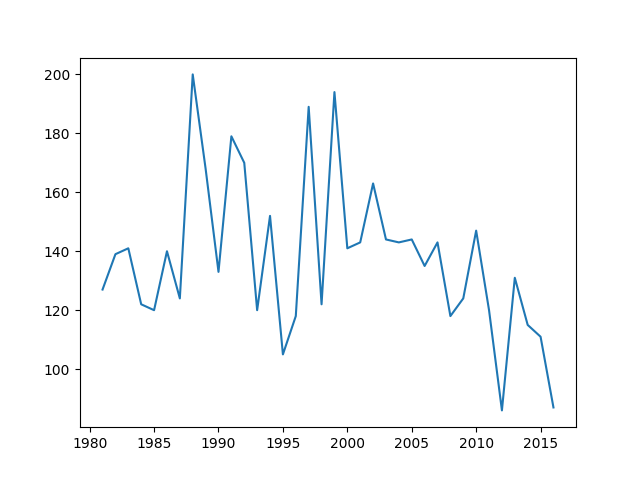
\includegraphics[scale=0.5]{trend.png}
\caption{The number of people drown per year}
\label{fig: label}
\end{figure}

We can see that the number of drown in Finland is decreasing.
\subsection*{Stan model}
\begin{minted}[bgcolor=bg, linenos, fontsize=\footnotesize]{python}  
stan_code = '''
data {
  int<lower=0> N; // number of data points
  vector[N] x;    // observation year
  vector[N] y;    // observation number of drowned
  real xpred;     // prediction year
  real tau;
}
parameters {
  real alpha;
  real beta;
  real<lower=0> sigma;
}
transformed parameters {
  vector[N] mu;
  mu = alpha + beta * x;
}
model {
  beta ~ normal(0, tau * tau);
  y ~ normal(mu, sigma);
}
generated quantities {
  real ypred;
  ypred = normal_rng(alpha + beta * xpred, sigma);
}
'''
\end{minted}
\textbf{Fix 1} In parameters, sigma has no lower bound and should be fixed by
\begin{minted}[bgcolor=bg, linenos, fontsize=\footnotesize]{python}  
real<lower=0> sigma;
\end{minted}
\textbf{Fix 2} In generated quantities, it aims to calculate for the prediction year and should be fixed by
 \begin{minted}[bgcolor=bg, linenos, fontsize=\footnotesize]{python}  
ypred = normal_rng(alpha + beta * xpred, sigma);
\end{minted}

The suitable numerical value presented for $\tau=26.6121$

\begin{minted}[bgcolor=bg, linenos, fontsize=\footnotesize]{bash} 
         mean se_mean     sd   2.5%    25%    50%    75%  97.5%  n_eff   Rhat
alpha  1804.1   24.67 840.37 171.67 1250.4 1786.9 2335.3 3506.5   1161    1.0
beta    -0.83    0.01   0.42  -1.68   -1.1  -0.83  -0.56  -0.02   1161    1.0
sigma    26.4    0.08   3.33  20.89  24.07  26.07  28.34  34.04   1640    1.0
mu[1]   152.4    0.23   8.51  135.9 146.86 152.33 157.86 169.86   1393    1.0
mu[2]  151.57    0.22   8.16 135.74 146.28 151.49 156.84 168.27   1421    1.0
						... ...
mu[36] 123.22    0.22    8.6 106.16 117.52 123.27 128.97 139.76   1485    1.0
ypred   121.0    0.46  27.14  68.54  102.4 120.68 139.68 174.54   3444    1.0
lp__   -131.8    0.04    1.2 -134.9 -132.4 -131.5 -130.9 -130.4   1072    1.0
\end{minted}

From the above table the the ypred is the prediction for 2019 which is 121

\begin{figure}[H]
\centering  
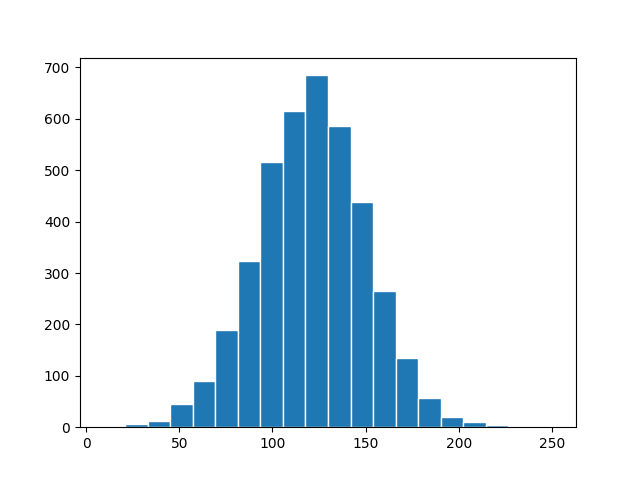
\includegraphics[scale=0.5]{hist.png}
\caption{The number of people drown per year}
\label{fig: label}
\end{figure}


\section{Hierarchical model: factory data with Stan}

\subsection{Separate model}

\begin{minted}[bgcolor=bg, linenos, fontsize=\footnotesize]{python}  
stan_code_separate = '''
data {
    int<lower=0> N;               // number of data points
    int<lower=0> K;               // number of groups
    int<lower=1,upper=K> x[N];    // group indicator
    vector[N] y;
}
parameters {
    vector[K] mu;                 // group means
    vector<lower=0>[K] sigma;     // group stds
}
model {
    y ~ normal(mu[x], sigma[x]);
}
generated quantities {
    real ypred;
    ypred = normal_rng(mu[6], sigma[6]);
}
'''
\end{minted}

\begin{minted}[bgcolor=bg, linenos, fontsize=\footnotesize]{bash}  
           mean se_mean     sd   2.5%    25%    50%    75%  97.5%  n_eff   Rhat
mu[1]     76.62     0.7  19.01  43.84  68.49  76.47  83.97 110.09    745    1.0
mu[2]    106.19    0.24   9.29   87.8 101.66 106.24 110.57 126.56   1557    1.0
mu[3]     87.24    0.42  10.69  65.71  82.54  87.72  92.73 106.98    645   1.01
mu[4]    111.75    0.18   6.44   99.6 108.51 111.57 114.55 125.91   1252    1.0
mu[5]     90.12    0.28   9.26  70.87  85.78  90.14  94.41 109.23   1116    1.0
mu[6]      86.1    0.36  14.32  56.76  78.74  86.31   93.5 115.39   1583    1.0
sigma[1]  32.31    0.86  24.94  12.65  19.46   25.7  36.74  95.36    837    1.0
sigma[2]  18.43    0.34   11.8   7.64  11.67  15.03  21.25  51.02   1212    1.0
sigma[3]  20.43    0.49  13.09   8.35  12.66  16.81   23.5  57.44    720    1.0
sigma[4]  12.35    0.27   8.78   4.99   7.52   10.0  14.04  33.83   1094    1.0
sigma[5]   17.5    0.35  11.64   7.14  10.76  14.15  20.01  48.24   1086    1.0
sigma[6]  29.34    0.47  17.23  12.54  18.86  24.72  34.16  74.79   1347    1.0
ypred     86.96    0.65  36.82  10.78   69.4  87.07  104.4 161.39   3187    1.0
lp__     -81.31    0.11   3.19 -88.67 -83.14 -80.92 -78.99 -76.24    899    1.0
\end{minted}

i) The posterior distribution of the mean of the quality measurements of the sixth machine.

$\mu_6=86.1$
\begin{minted}[bgcolor=bg, linenos, fontsize=\footnotesize]{python}
fit_separate = model_seperate.sampling(data=data_separate, n_jobs=-1)
mu_data_separate = fit_separate.extract()['mu']
\end{minted}

\begin{figure}[H]
\centering  
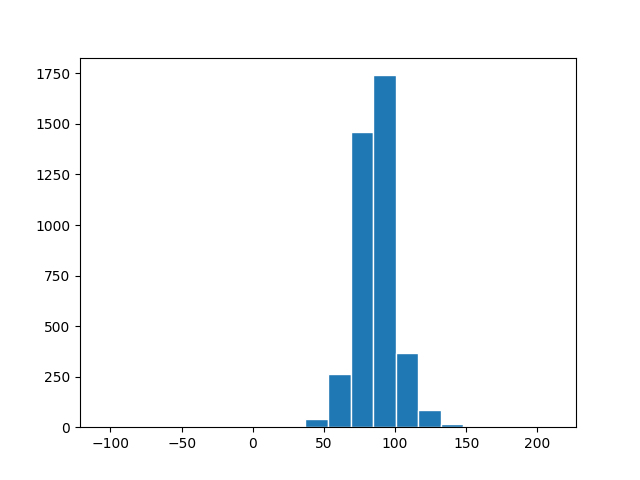
\includegraphics[scale=0.5]{separate_hist_mu_six.png}
\caption{$\mu$ histogram}
\label{fig: label}
\end{figure}

ii) The predictive distribution for another quality measurement of the sixth machine.

\begin{minted}[bgcolor=bg, linenos, fontsize=\footnotesize]{python}
fit_separate = model_seperate.sampling(data=data_separate, n_jobs=-1)
y_pred_separate = fit_separate.extract()['ypred']  
\end{minted}


\begin{figure}[H]
\centering  
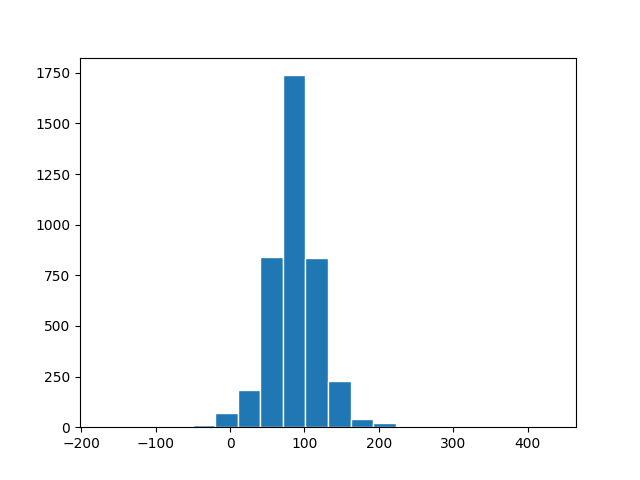
\includegraphics[scale=0.5]{separate_hist.png}
\caption{Prediction histogram}
\label{fig: label}
\end{figure}

iii) The posterior distribution of the mean of the quality measurements of the seventh machine.

In the separate model we treat each machine separately. Since we don't have information about the seventh machine. Thus we cannot tell its posterior distribution.

\subsection{pooled model}

\begin{minted}[bgcolor=bg, linenos, fontsize=\footnotesize]{python}  
stan_code_pooled = '''
data {
    int<lower=0> N;       // number of data points
    vector[N] y;          //
}
parameters {
    real mu;              // group means
    real<lower=0> sigma;  // common std
}
model {
    y ~ normal(mu, sigma);
}
generated quantities {
    real ypred;
    ypred = normal_rng(mu, sigma);
}
'''
\end{minted}

\begin{minted}[bgcolor=bg, linenos, fontsize=\footnotesize]{bash}  
        mean se_mean     sd   2.5%    25%    50%    75%  97.5%  n_eff   Rhat
mu     92.99    0.06   3.53  86.23  90.54  93.01  95.32 100.04   2953    1.0
sigma  18.83    0.05   2.54   14.6  17.06  18.55  20.36  24.63   3023    1.0
ypred  93.43    0.31  19.54  55.75  80.25  93.81 106.42  130.8   3953    1.0
lp__  -99.34    0.02   1.01 -102.0 -99.73 -99.05 -98.62 -98.34   1806    1.0
\end{minted}

i) The posterior distribution of the mean of the quality measurements of the sixth machine.

For the pooled model, all the machines are considered as an entity, thus all the measurements are combined into one and performed prediction on the whole data. $\mu$ will be the same for all the machines.

\begin{minted}[bgcolor=bg, linenos, fontsize=\footnotesize]{python}  
fit_pooled = model_pooled.sampling(data=data_pooled)
mu = fit_pooled.extract()['mu']
\end{minted}

\begin{figure}[H]
\centering  
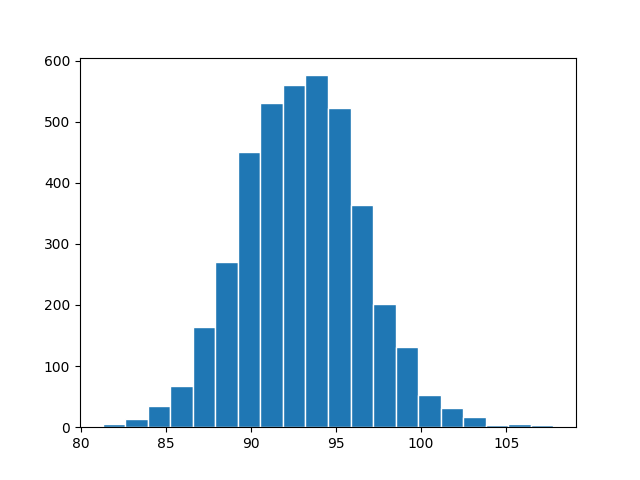
\includegraphics[scale=0.5]{pooled_hist_mu.png}
\caption{Prediction histogram}
\label{fig: label}
\end{figure}

ii) The predictive distribution for another quality measurement of the sixth machine.

\begin{minted}[bgcolor=bg, linenos, fontsize=\footnotesize]{python}  
fit_pooled = model_pooled.sampling(data=data_pooled)
y_pred_pooled = fit_pooled.extract()['ypred']
\end{minted}

\begin{figure}[H]
\centering  
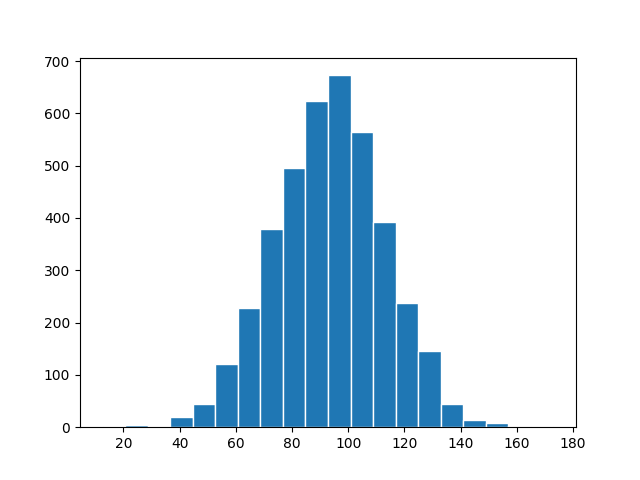
\includegraphics[scale=0.5]{pooled_hist.png}
\caption{Prediction histogram}
\label{fig: label}
\end{figure}

iii) The posterior distribution of the mean of the quality measurements of the seventh machine.

For the pooled model, all the machines are considered as an entity, thus all the measurements are combined into one and performed prediction on the whole data. The posterior distribution of the mean of the quality measurements of the seventh machine is equal to that of the sixth machine.


\subsection{Hierarchical model}

\begin{minted}[bgcolor=bg, linenos, fontsize=\footnotesize]{python}  
stan_code_hierarchical = '''
data {
    int<lower=0> N;             // number of data points
    int<lower=0> K;             // number of groups
    int<lower=1,upper=K> x[N];  // group indicator
    vector[N] y;
}
parameters {
    real mu0;                   // prior mean
    real<lower=0> sigma0;       // prior std
    vector[K] mu;               // group means
    real<lower=0> sigma;        // common std
}
model {
    mu ~ normal(mu0, sigma0);
    y ~ normal(mu[x], sigma);
}
generated quantities {
    real ypred6;
    real mu7;
    ypred6 = normal_rng(mu[6], sigma);
    mu7 = normal_rng(mu0, sigma0);
}
'''
\end{minted}


\begin{minted}[bgcolor=bg, linenos, fontsize=\footnotesize]{bash}  
         mean se_mean     sd   2.5%    25%    50%    75%  97.5%  n_eff   Rhat
mu0     92.96    0.27   9.11  77.19  88.49  92.97  97.37 109.84   1122    1.0
sigma0   16.2    0.33  10.13   4.18  10.21  14.02  19.23  41.65    928    1.0
mu[1]   79.85    0.18   6.91  66.07  75.28   79.8  84.49  92.89   1467    1.0
mu[2]  103.08    0.26   6.77  88.38  98.76 103.18 107.48 116.39    677    1.0
mu[3]   89.05    0.11   6.17  76.57  85.04   89.2  93.19 101.16   3223    1.0
mu[4]  107.11    0.29   7.13  91.57 102.47 107.58 111.89 120.77    607    1.0
mu[5]    90.6     0.1   5.95  78.46  86.91   90.6  94.42  102.4   3606    1.0
mu[6]   87.54    0.11   6.14   75.3  83.45  87.76  91.68  99.85   3297    1.0
sigma   15.24    0.08   2.39  11.36  13.54  14.93  16.65  20.54    941    1.0
ypred6  87.32    0.26  16.48  54.75  76.32   87.2  98.16 120.36   4099    1.0
mu7      92.7    0.43  22.23  51.61  82.94  92.81 102.74 133.11   2670    1.0
lp__   -108.8    0.07   2.49 -114.6 -110.2 -108.4 -107.0 -105.2   1377    1.0
\end{minted}


i) The posterior distribution of the mean of the quality measurements of the sixth machine.

The hierarchical model not only treats every machine separately, but also computes the combination of all the machines as one entity. $\mu_6=87.54$

\begin{figure}[H]
\centering  
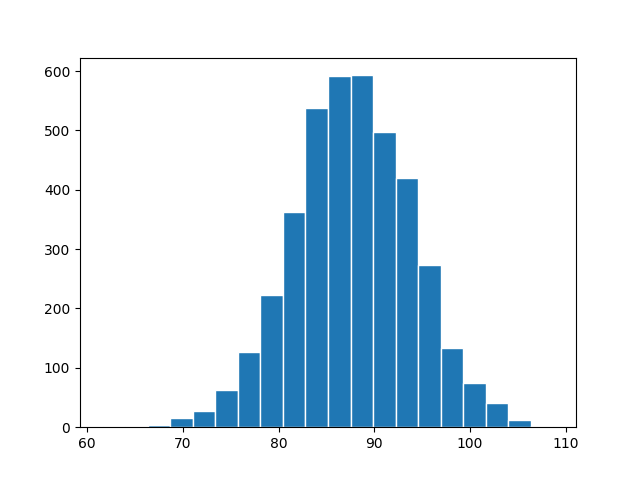
\includegraphics[scale=0.5]{hierarchical_hist_mu_six.png}
\caption{Prediction histogram}
\label{fig: label}
\end{figure}

ii) The predictive distribution for another quality measurement of the sixth machine.

\begin{minted}[bgcolor=bg, linenos, fontsize=\footnotesize]{python}  
fit_hierarchical = model_hierarchical.sampling(data=data_hierarchical, n_jobs=-1)
mu_data_hierarchical = fit_hierarchical.extract()['mu']
\end{minted}

\begin{figure}[H]
\centering  
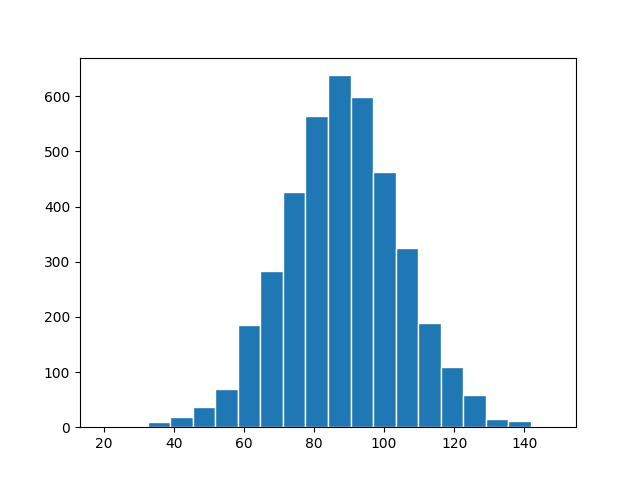
\includegraphics[scale=0.5]{hierarchical_hist.png}
\caption{Prediction histogram}
\label{fig: label}
\end{figure}

iii) The posterior distribution of the mean of the quality measurements of the seventh machine.

The hierarchical model not only treats every machine separately, but also computes the combination of all the machines as one entity. It can predict measurements for the machines even without data. we can plot the histogram:
$\mu_7=92.7$

\begin{minted}[bgcolor=bg, linenos, fontsize=\footnotesize]{python}  
fit_hierarchical = model_hierarchical.sampling(data=data_hierarchical, n_jobs=-1)
mu_data_hierarchical_7 = fit_hierarchical.extract()['mu7']
\end{minted}

\begin{figure}[H]
\centering  
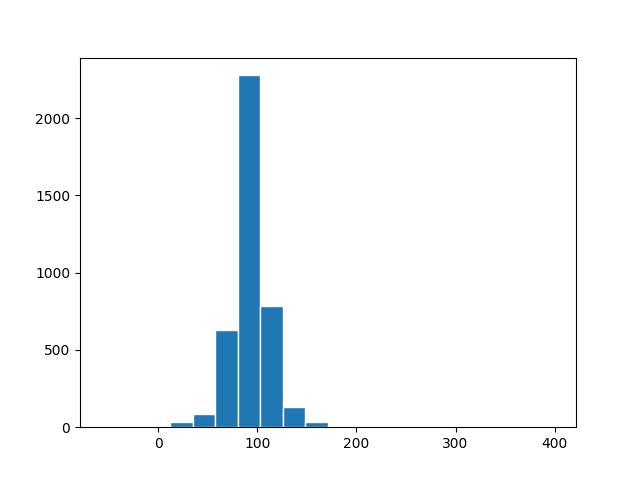
\includegraphics[scale=0.5]{hierarchical_hist_mu_seven.png}
\caption{Prediction histogram}
\label{fig: label}
\end{figure}



\appendix
\section{Exercise 1}

\begin{minted}[bgcolor=bg, linenos, fontsize=\footnotesize]{python}  
import matplotlib
from scipy.stats import norm
import matplotlib.pyplot as plt
import numpy as np
import pandas as pd
import pystan

drowning_data = pd.read_fwf('./drowning.txt').values
years = drowning_data[:, 0]
drowning = drowning_data[:, 1]

print("mean:", np.mean(drowning))
print("standard deviation:", np.std(drowning,ddof=1))

plt.plot(years, drowning)
plt.savefig('./trend.png')
plt.show()

stan_code = '''
data {
  int<lower=0> N; // number of data points
  vector[N] x;    // observation year
  vector[N] y;    // observation number of drowned
  real xpred;     // prediction year
  real tau;
}
parameters {
  real alpha;
  real beta;
  real<lower=0> sigma;
}
transformed parameters {
  vector[N] mu;
  mu = alpha + beta * x;
}
model {
  beta ~ normal(0, tau*tau);
  y ~ normal(mu, sigma);
}
generated quantities {
  real ypred;
  ypred = normal_rng(alpha + beta * xpred, sigma);
}
'''

stan_model = pystan.StanModel(model_code=stan_code)

data = dict(
    N=len(years),
    x=years,
    y=drowning,
    xpred=2019,
    tau=26.612146647843897,
)

fit = stan_model.sampling(data=data)
print(fit)

y_pred = fit.extract()['ypred']
plt.hist(y_pred, bins=20, ec='white')
plt.savefig('./hist.png')
plt.show()

\end{minted}

\section{Exercise 2}

\begin{minted}[bgcolor=bg, linenos, fontsize=\footnotesize]{python}  
import matplotlib
from scipy.stats import norm
import matplotlib.pyplot as plt
import numpy as np
import pandas as pd
import pystan

machines = pd.read_fwf('./factory.txt', header=None).values
machines_transposed = machines.T


stan_code_separate = '''
data {
    int<lower=0> N;               // number of data points
    int<lower=0> K;               // number of groups
    int<lower=1,upper=K> x[N];    // group indicator
    vector[N] y;
}
parameters {
    vector[K] mu;                 // group means
    vector<lower=0>[K] sigma;     // group stds
}
model {
    y ~ normal(mu[x], sigma[x]);
}
generated quantities {
    real ypred;
    ypred = normal_rng(mu[6], sigma[6]);
}
'''

model_seperate = pystan.StanModel(model_code=stan_code_separate)
data_separate = dict(
    N=machines_transposed.size,
    K=6,
    x=[
        1, 1, 1, 1, 1,
        2, 2, 2, 2, 2,
        3, 3, 3, 3, 3,
        4, 4, 4, 4, 4,
        5, 5, 5, 5, 5,
        6, 6, 6, 6, 6,
    ],
    y=machines_transposed.flatten()
)

fit_separate = model_seperate.sampling(data=data_separate, n_jobs=-1)
print(fit_separate)

y_pred_separate = fit_separate.extract()['ypred']
plt.hist(y_pred_separate, bins=20, ec='white')
plt.savefig('./separate_hist.png')
plt.show()

mu_data_separate = fit_separate.extract()['mu']
plt.hist(mu_data_separate[:, 5], bins=20, ec='white')
plt.savefig('./separate_hist_mu_six.png')
plt.show()

stan_code_pooled = '''
data {
    int<lower=0> N;       // number of data points
    vector[N] y;          //
}
parameters {
    real mu;              // group means
    real<lower=0> sigma;  // common std
}
model {
    y ~ normal(mu, sigma);
}
generated quantities {
    real ypred;
    ypred = normal_rng(mu, sigma);
}
'''

machines_pooled = machines.flatten()
model_pooled = pystan.StanModel(model_code=stan_code_pooled)
data_pooled = dict(
    N=machines_pooled.size,
    y=machines_pooled
)

fit_pooled = model_pooled.sampling(data=data_pooled)
print(fit_pooled)

y_pred_pooled = fit_pooled.extract()['ypred']
plt.hist(y_pred_pooled, bins=20, ec='white')
plt.savefig('./pooled_hist.png')
plt.show()

mu = fit_pooled.extract()['mu']
plt.hist(mu, bins=20, ec='white')
plt.savefig('./pooled_hist_mu.png')
plt.show()

stan_code_hierarchical = '''
data {
    int<lower=0> N;             // number of data points
    int<lower=0> K;             // number of groups
    int<lower=1,upper=K> x[N];  // group indicator
    vector[N] y;
}
parameters {
    real mu0;                   // prior mean
    real<lower=0> sigma0;       // prior std
    vector[K] mu;               // group means
    real<lower=0> sigma;        // common std
}
model {
    mu ~ normal(mu0, sigma0);
    y ~ normal(mu[x], sigma);
}
generated quantities {
    real ypred6;
    real mu7;
    ypred6 = normal_rng(mu[6], sigma);
    mu7 = normal_rng(mu0, sigma0);
}
'''

model_hierarchical = pystan.StanModel(model_code=stan_code_hierarchical)
data_hierarchical = dict(
    N=machines_transposed.size,
    K=6,
    x=[
        1, 1, 1, 1, 1,
        2, 2, 2, 2, 2,
        3, 3, 3, 3, 3,
        4, 4, 4, 4, 4,
        5, 5, 5, 5, 5,
        6, 6, 6, 6, 6,
    ],
    y=machines_transposed.flatten()
)

fit_hierarchical = model_hierarchical.sampling(data=data_hierarchical, n_jobs=-1)
print(fit_hierarchical)

mu_data_hierarchical = fit_hierarchical.extract()['mu']
plt.hist(mu_data_hierarchical[:, 5], bins=20, ec='white')
plt.savefig('./hierarchical_hist_mu_six.png')
plt.show()

y_pred_hierarchical = fit_hierarchical.extract()['ypred6']
plt.hist(y_pred_hierarchical, bins=20, ec='white')
plt.savefig('./hierarchical_hist.png')
plt.show()

mu_data_hierarchical_7 = fit_hierarchical.extract()['mu7']
plt.hist(mu_data_hierarchical_7, bins=20, ec='white')
plt.savefig('./hierarchical_hist_mu_seven.png')
plt.show()

\end{minted}

\end{document}